\chapter{Análisis del problema}
\section{Descripción del problema a resolver}

El envejecimiento progresivo de la población ha incrementado significativamente la prevalencia de enfermedades neurodegenerativas, siendo el Alzheimer la principal causa de demencia a nivel mundial. Esta enfermedad se caracteriza por un deterioro cognitivo gradual que afecta a la memoria, el lenguaje, la orientación y las funciones ejecutivas, limitando progresivamente la autonomía de quienes la padecen. Aunque no existe un tratamiento curativo, la estimulación cognitiva ha demostrado ser eficaz para ralentizar el deterioro y preservar las capacidades intelectuales durante más tiempo.

Actualmente existen aplicaciones comerciales de estimulación cognitiva, pero presentan barreras importantes que limitan su alcance. Plataformas como Constant Therapy, analizada en el capítulo anterior, ofrecen programas de rehabilitación con respaldo científico, sin embargo su uso está condicionado por sus elevados costes de suscripción, su orientación exclusiva al mercado angloparlante y una interfaz optimizada principalmente para dispositivos móviles que no siempre resulta accesible para el perfil de usuario mayor. Además, estas soluciones no permiten una supervisión directa por parte de terapeutas ni la personalización de las actividades según las necesidades específicas de cada paciente.

El problema que aborda este proyecto es la ausencia de una plataforma web gratuita, accesible desde ordenadores de sobremesa y adaptada al contexto español, que integre ejercicios de estimulación cognitiva validados científicamente con un sistema de gestión clínica que permita a los terapeutas asignar actividades personalizadas y realizar un seguimiento objetivo del progreso de sus pacientes. La solución debe estar diseñada específicamente para personas mayores, con una interfaz sencilla e intuitiva que minimice la carga cognitiva y facilite la interacción independiente.

\section{Requisitos funcionales}
En esta sección se definen las diferentes funcionalidades de la aplicación web que son necesarias para cubrir las diferentes necesidades de los usuarios. Las he dividido de la siguiente manera:  
\begin{itemize}
    \item \textbf{RF-1. Gestión de usuarios.}
    \begin{itemize}
        \item \textbf{RF-1.1.} El usuario administrador dará de alta a los distintos terapeutas.
        \item \textbf{RF-1.2.} El usuario terapeuta dará de alta al usuario paciente.
        \item \textbf{RF-1.3.} El usuario administrador podrá modificar sus propios datos.
        \item \textbf{RF-1.4.} El usuario administrador podrá modificar los datos del usuario terapeuta tales como: Nombre, Apellidos, teléfono de contacto, Email.
        \item \textbf{RF-1.5.} El usuario terapeuta podrá modificar los datos del usuario paciente tales como: Nombre, Apellidos, teléfono de contacto y en su caso si hubiera de su cuidador o cuidadora.
        \item \textbf{RF-1.6.} El usuario terapeuta dará de baja a los usuarios pacientes.
        \item \textbf{RF-1.7.} El usuario administrador dará de baja a los usuarios terapeutas.
        \item \textbf{RF-1.8.} El usuario terapeuta podrá ver la información de sus usuarios pacientes.
        \item \textbf{RF-1.9.} Todos los usuarios podrán iniciar sesión con su usuario y contraseña.
    \end{itemize}

    
    \item \textbf{RF-2. Asignación de pacientes.} 
    \begin{itemize}
        \item \textbf{RF-2.1.} El usuario terapeuta será el que asigne sus propios pacientes dentro de la aplicación.
    \end{itemize}
    
    \item \textbf{RF-3. Gestión de agenda de pacientes.}
    \begin{itemize}
        \item \textbf{RF-3.1.} Los usuarios pacientes serán mostrados al usuario terapeuta.
        \item \textbf{RF-3.2.} El usuario terapeuta podrá ver la agenda de sus usuarios pacientes.
        \item \textbf{RF-3.3.} El usuario terapeuta podrá ver los juegos disponibles.
        \item \textbf{RF-3.4.} El usuario terapeuta podrá editar las agendas de los pacientes.
        \item \textbf{RF-3.5.} El usuario terapeuta habilitará los juegos a sus usuarios pacientes.
        \item \textbf{RF-3.6.} El usuario paciente podrá ver los juegos que le han sido asignados o le quedan por hacer.
        \item \textbf{RF-3.7.} El usuario terapeuta seleccionará el juego o los juegos a asignar a cada usuario paciente.
    \end{itemize}
    
    \item \textbf{RF-5. Juegos.} 
    Esta parte de los requisitos funcionales se encarga de describir los juegos que se implementarán en la aplicación.
    \begin{itemize}
        \item \textbf{RF-5.1.} Cada juego irá acompañado de una descripción breve y detallada de cómo funciona, además de un audio explicativo.  
        \item \textbf{RF-5.2.} Ordenar la secuencia, consistirá en replicar una secuencia breve de imágenes visualizadas anteriormente durante un periodo de tiempo.
        \item \textbf{RF-5.3.} Objetos, establecimiento y profesionales.
        \item \textbf{RF-5.4.} Pagos exactos, consistirá en devolver la cantidad de monedas o billetes, dado un número, acompañado de imágenes de los billetes y monedas para que el usuario haga clic sobre las que necesite.
        \item \textbf{RF-5.5.} Vístete, consistirá en unir las prendas de ropa que se muestren con la parte del cuerpo que corresponda; al lado de las prendas aparecerá una silueta de un cuerpo humano.
        \item \textbf{RF-5.6.} Completar la oración, el usuario leerá una oración incompleta, y deberá elegir entre dos opciones, para que la oración tenga sentido.
        \item \textbf{RF-5.7.} El intruso, el usuario deberá elegir la palabra intrusa entre tres posibilidades, de las cuales dos están relacionadas y la otra no tiene nada que ver.
    \end{itemize}
    
    \item \textbf{RF-6. Gestión de estadísticas.}
    \begin{itemize}
        \item \textbf{RF-6.1.} El usuario terapeuta podrá consultar el número de errores y el tiempo que ha tardado el usuario en realizar un juego.
        \item \textbf{RF-6.2.} El usuario paciente podrá revisar sus estadísticas.
        \item \textbf{RF-6.3.} El usuario terapeuta podrá exportar un archivo .xls, donde verá todas las estadísticas de sus pacientes.
    \end{itemize}
    
    \item \textbf{RF-7. Narrativa y recompensas.}
    \begin{itemize}
        \item \textbf{RF-7.1.} El programa mostrará una pequeña historia relacionada como introducción a cada ejercicio que se realice, con el objetivo de mantener la atención y motivación del usuario.
        \item \textbf{RF-7.2.} Por cada semana que se hayan completado los juegos correctamente, el usuario recibirá una insignia en señal de su esfuerzo.
    \end{itemize}

\end{itemize}


\section{Requisitos no funcionales}
En este apartado se describen los requisitos no funcionales de la aplicación. Donde se tratará la usabilidad, la accesibilidad, el rendimiento y la información.
\begin{itemize}
    \item \textbf{RNF-1. Usabilidad.}  Al ser un juego orientado para personas de edad avanzada y con principios de alzheimer, la interacción con la aplicación será sencilla e intuitiva.
    \begin{itemize}
        \item \textbf{RNF-1.1.} La aplicación garantizará una interfaz sencilla y simple para evitar la sobrecarga cognitiva.
        \item \textbf{RNF-1.2.} Las instrucciones serán claras y concisas.
        \item \textbf{RNF-1.3.} La navegación será muy intuitiva para que los usuarios no tengan confusiones.
        \item \textbf{RNF-1.4.} Uso de iconos para mejorar la interfaz y hacerla mas intuitiva.
    \end{itemize}
    \item \textbf{RNF-2. Accesibilidad.} Es una de las partes más esenciales de la aplicación, debido a que esta orientado a personas de edad avanzada.
    \begin{itemize}
        \item \textbf{RNF-2.1.} El sistema no usará ni micrófono ni cámara.
        \item \textbf{RNF-2.2.} Tamaño de letra y tamaño de botones grande para facilitar la lectura y la interacción.
        \item \textbf{RNF-2.3.} Mensajes de error en caso de errar en alguna tarea.
        \item \textbf{RNF-2.4.} El diseño de la aplicación será adaptable.
    \end{itemize}
    \item \textbf{RNF-3.} Rendimiento. 
    \begin{itemize}
        \item \textbf{RNF-3.1.} Se deben minimizar la aparición de errores, para garantizar el buen funcionamiento del juego.
        \item \textbf{RNF-3.2} Las respuestas del juego deben ser rápidas y precisas para poder generar fluidez en la experiencia del usuario.
        \item \textbf{RNF-3.3} El sistema debe ser capaz de soportar varios usuarios a la vez.
    \end{itemize}
    \item \textbf{RNF-4. Información.} 
    \begin{itemize}
        \item \textbf{RNF-4.1.} La plataforma contará con un sistema de logs para el monitoreo de actividad.
        \item \textbf{RNF-4.2.} La información de los pacientes se guardará de forma encriptada para asegurar la privacidad de los datos.
        
    \end{itemize}
    \item  \textbf{RNF-5. Seguridad.}
    \begin{itemize}
        \item \textbf{RNF-5.1.} La aplicación deberá seguir las instrucciones basadas en el principio de mínimo privilegio al utilizar AWS.
    \end{itemize}
    \item \textbf{RNF-6. Compatibilidad.}
    \begin{itemize}
        \item \textbf{RNF-6.1} El sistema será compatible con dispositivos táctiles como tablets o smartphones.
    \end{itemize}
\end{itemize}

\section{Casos de uso}
Para el desarrollo de la aplicación aplicación y conseguir un prototipo de funcionamiento de esta, varios diagramas de casos de uso han sido realizados  para cada uno de los apartados de los requisitos de uso (registro de usuarios, asignación de pacientes,gestión de agenda de pacientes, gestión de estadísticas y narrativa y recompensas). La parte de juegos no esta contemplada debido a que esto tiene más que ver con la implementación que con el análisis.

\subsection{Actores del sistema}
Tras analizar y revisar los requisitos, he determinado que haya tres roles en el sistema. Habrá tres roles, uno de ellos será el administrador del sistema, otro de ellos el usuario terapeuta, y por último el usuario paciente, no habrá más roles a considerar que sean relevantes.


\begin{table}[H]
    \centering
    \begin{tabular}{|p{3cm}|p{6cm}|p{2cm}|} 
        \hline
        \textbf{Actor} & Administrador del sistema & ACT\_1 \\ 
        \hline
        \textbf{Descripción} & \multicolumn{2}{|p{8cm}|}{Usuario con todos los privilegios del sistema} \\ 
        \hline
        \textbf{Características} & \multicolumn{2}{|p{8cm}|}{Perfil destinado a los usuarios que dan de alta a los usuarios terapeutas} \\ 
        \hline
        \textbf{Relaciones} & \multicolumn{2}{|p{8cm}|}{RF-1.1} \\ 
        \hline
    \end{tabular}
    \label{tab:Actor Administrador}
\end{table}


\begin{table}[H]
    \centering
    \begin{tabular}{|p{3cm}|p{6cm}|p{2cm}|}
        \hline
        \multicolumn{3}{|l|}{\textbf{Atributos}} \\       
        \hline
        \textbf{Nombre} & \textbf{Descripción} & \textbf{Tipo} \\
        \hline
        Identificador & Identificador de la persona & Int \\  
        \hline
        Nombre & Nombre de la persona & String\\ 
        \hline
        Apellidos & Apellidos de la persona & String \\ 
        \hline
        Email & Email del usuario & String \\ 
        \hline
        Contraseña & Contraseña del usuario & String \\ 
        \hline
        Nombre de usuario & Nombre del usuario identificativo para iniciar sesión & String \\ 
        \hline
    \end{tabular}
    \caption{Descripción del usuario administrador}
    \label{tab:administrador_atributos}
\end{table}

\begin{table}[H]
    \centering
    \begin{tabular}{|p{3cm}|p{6cm}|p{2cm}|} 
        \hline
        \textbf{Actor} & Usuario terapeuta & ACT\_2 \\ 
        \hline
        \textbf{Descripción} & \multicolumn{2}{|p{8cm}|}{Usuario con priveligios sobre el paciente} \\ 
        \hline
        \textbf{Características} & \multicolumn{2}{|p{8cm}|}{Perfil destinado a los usuarios terapeutas, que supervisan a los pacientes} \\ 
        \hline
        \textbf{Relaciones} & \multicolumn{2}{|p{8cm}|}{RF-1.2,RF-1.3,RF-1.4,RF-2.1,RF-3.2,RF-3.3,RF-3.4,RF-3.5,RF-3.6,RF-5.1,RF-5.3} \\ 
        \hline
    \end{tabular}
    \label{tab:Actor terapeuta}
\end{table}
\begin{table}[H]
    \centering
    \begin{tabular}{|p{3cm}|p{6cm}|p{2cm}|}
        \hline
        \multicolumn{3}{|l|}{\textbf{Atributos}} \\       
        \hline
        \textbf{Nombre} & \textbf{Descripción} & \textbf{Tipo} \\
        \hline
        Identificador & Identificador de la persona & Int \\  
        \hline
        Nombre & Nombre de la persona & String\\ 
        \hline
        Apellidos & Apellidos de la persona & String \\ 
        \hline
        Email & Email del usuario & String \\ 
        \hline
        Contraseña & Contraseña del usuario & String \\ 
        \hline
        Nombre de usuario & Nombre del usuario identificativo para iniciar sesión & String \\ 
        \hline
    \end{tabular}
    \caption{Descripción del usuario terapeuta}
    \label{tab:terapeuta_atributos}
\end{table}
\begin{table}[H]
    \centering
    \begin{tabular}{|p{3cm}|p{6cm}|p{2cm}|} 
        \hline
        \textbf{Actor} & Usuario paciente & ACT\_3 \\ 
        \hline
        \textbf{Descripción} & \multicolumn{2}{|p{8cm}|}{Usuario destinado a realizar los juegos} \\ 
        \hline
        \textbf{Características} & \multicolumn{2}{|p{8cm}|}{Perfil destinado a realizar los juegos que les son propuestos} \\ 
        \hline
        \textbf{Relaciones} & \multicolumn{2}{|p{8cm}|}{RF-3.6,RF-5.2,RF-5.3,RF-5.4,RF-5.5,RF-5.6,RF-5.7,RF-4} \\ 
        \hline
    \end{tabular}
    \label{tab:Actor paciente}
\end{table}
\begin{table}[H]
    \centering
    \begin{tabular}{|p{3cm}|p{6cm}|p{2cm}|}
        \hline
        \multicolumn{3}{|l|}{\textbf{Atributos}} \\       
        \hline
        \textbf{Nombre} & \textbf{Descripción} & \textbf{Tipo} \\
        \hline
        Identificador & Identificador de la persona & Int \\  
        \hline
        Nombre & Nombre de la persona & String\\ 
        \hline
        Apellidos & Apellidos de la persona & String \\ 
        \hline
        Email & Email del usuario & String \\ 
        \hline
        Contraseña & Contraseña del usuario & String \\ 
        \hline
        Nombre de usuario & Nombre del usuario identificativo para iniciar sesión & String \\ 
        \hline
        Identificador terapueta & Identificador del terapeuta que lo supervisa & Int \\ 
        \hline
        Fecha de nacimiento & Fecha de nacimiento del usuario & Date \\ 
        \hline
    \end{tabular}
    \caption{Descripción del usuario paciente}
    \label{tab:paciente_atributos}
\end{table}

\section{Diagramas de casos de uso}
A continuación, se muestran los diagramas de casos de uso para cada uno de los 
apartados:

\begin{itemize}
    \item \textbf{Gestión de usuarios.}
    Como vemos en la figura 4.1, el administrador del sistema podrá dar de alta y baja
     a los usuarios terapeutas, y estos a su vez podrán dar de alta y baja a los 
     usuarios pacientes.
      Además, todos los usuarios podrán iniciar sesión, pero para que los datos del paciente solo podrá modificarlos el terapeuta y de la misma forma el terapeuta
      el cuál no tendrá forma autónoma de editar sus propios datos, lo hará el adminstrador .
     \begin{figure}[H]
    \centering
    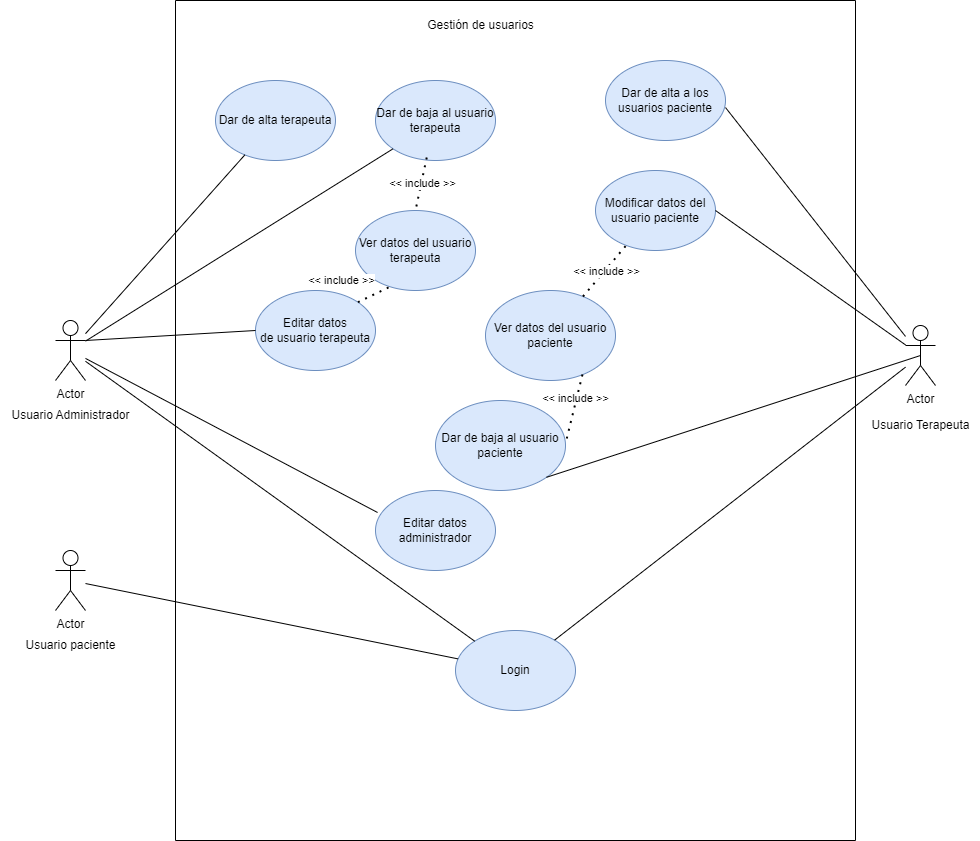
\includegraphics[width=0.8\textwidth]{imagenes/casos_uso/gestion_usuarios.png}
    \caption{Diagrama de casos de uso: Gestión de usuarios}
\end{figure}

\item \textbf{Asignación de pacientes:} Como comprobamos en la figura 4.2, el usuario terapeuta 
será el que asigne sus propios pacientes dentro de la aplicación. Así, el terapeuta podrá ver 
la lista de pacientes que tiene asignados y podrá asignar nuevos pacientes a su lista.
\begin{figure}[H]
    \centering
    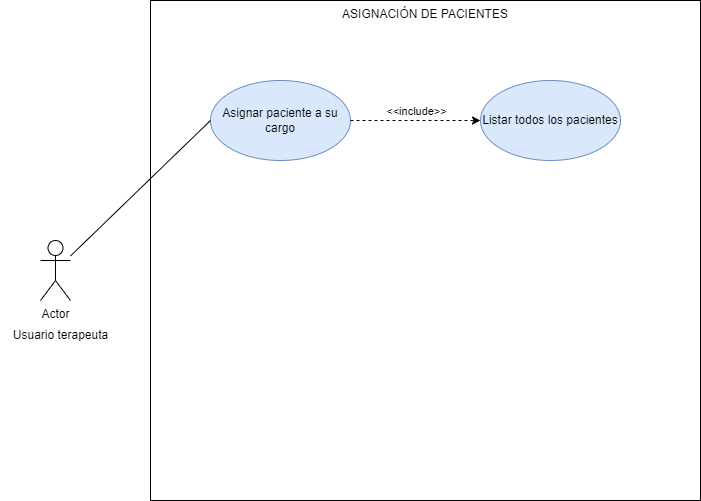
\includegraphics[width=0.6\textwidth]{imagenes/casos_uso/asignacion_pacientes.png}
    \caption{Diagrama de casos de uso: Asignación de pacientes}
\end{figure}

\item \textbf{Gestión de agendas de pacientes:} En la figura 4.3, podemos observar que el usuario 
terapeuta podrá ver la agenda de sus usuarios pacientes, así como los juegos disponibles.
 Además, el terapeuta podrá editar las agendas de los pacientes, habilitando los juegos a sus 
 usuarios pacientes. Por otro lado, el usuario paciente podrá ver los juegos que le han sido 
 asignados o le quedan por hacer.

 \item \textbf{Gestión de estadísticas:} En la figura 4.4, el usuario terapeuta podrá consultar
  el número de errores y el tiempo que ha tardado el usuario en realizar un juego.
    Además, el usuario paciente podrá revisar sus estadísticas, y el terapeuta podrá exportar
     un archivo .xls, donde verá todas las estadísticas de sus pacientes.
    \begin{figure}[H]
    \centering
    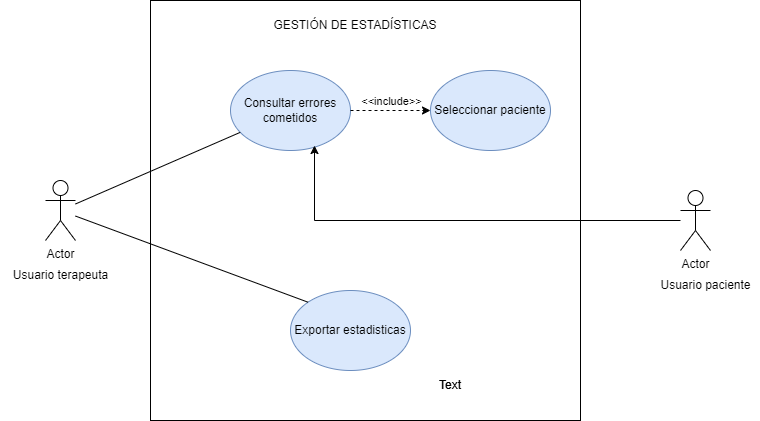
\includegraphics[width=0.8\textwidth]{imagenes/casos_uso/gestion_estadisticas.png}
    \caption{Diagrama de casos de uso: Gestión de estadísticas}
\end{figure}
\end{itemize}
